\subsection{Known Problems}

The following sections discusses some of the problems I faced, and solutions or mitigations I employed.

\paragraph{Incorrect Ultrasonic Measurements during \IIC communication}
During an earlier stage of the project, Ultrasonic measurement received immediately after Gyroscope reading were off
by a lot.
While this does not seem to be an issue anymore, I am neither sure what caused this nor why it works now.
Potential mitigation strategies for this would have been laptop sided, were values received right after gyroscope data
could either be dropped or substituted by a suitable average.


\paragraph{Unknown path width}
Classification could be much simpler if path width was known. Three distance measurements would suffice for classification, one at 0, one at 90 and one at 180 Degrees.
A X Junction would have all three measurements larger than path width,
T Junction would have first and third measurement larger, second measurement equal to path width (technically more like half path width) and
a corridor would just have the second measurement greater than path width.
My first idea was to use the distance measurements at $45\deg$ and $135\deg$, where the corners would be expected for a X Junction, to estimate this variable.
This did not turn out to be a workable approach for several reasons.
First, the ultrasonic sensor fails to get reliable readings for the distance if the object is at too much of an angle.
Secondly, this approach would only be useful for X-Junctions, as the other two types do not have the corners necessary.

This did not turn out to be a problem after all, since classification now works based on similarity to past data and should due to normalization be somewhat independent of path width.

\paragraph{Graphing the environment from the scan data} Probably as a result of the difficulty to get measurements at an angle, the data cannot be easily graphed to show the scanned environment.
Considering our data consists of angles and distances, it can be understood as polar coordinates.
Therefore, converting it to cartesian coordinates and plotting those should give a pretty good image of the junction.
This works very well in theory, but not as well with values actually measured by the sensors, see Figure \ref{fig:cartesian}.
This is not of much importance to the overall project, but would have been helpful for visualization.

\begin{figure}[H]
    \centering
    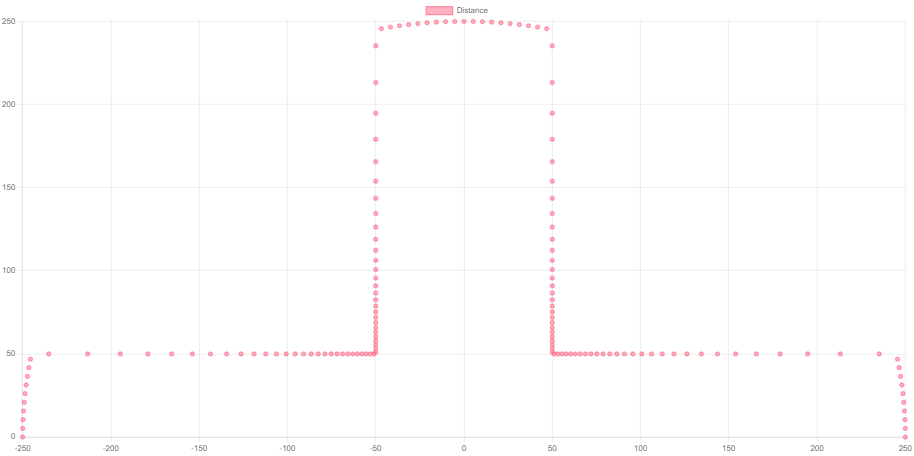
\includegraphics[width=0.45\linewidth]{figures/cartesian_simulated.png}
    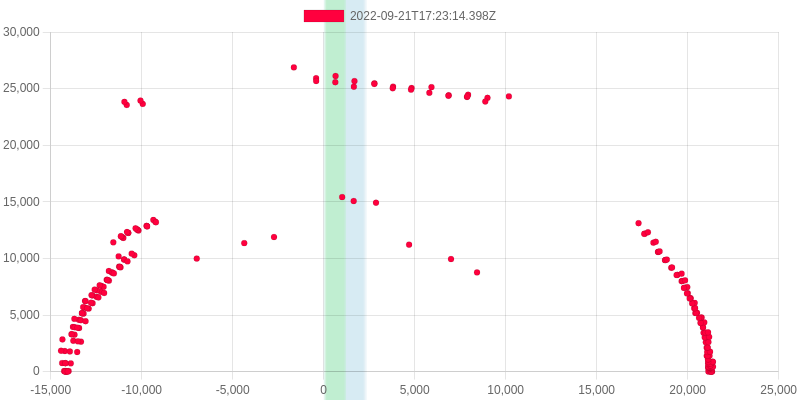
\includegraphics[width=0.45\linewidth]{figures/cartesian_actual.png}
    \caption{Left: simulated data, converted to cartesian coordinates and
        graphed.
        Right: actual data, converted to cartesian coordinates and graphed.
        Notice the missing sections, that are mostly obstacles at an angle.}

    \label{fig:cartesian}
\end{figure}

\paragraph{Turns are not detected correctly} When a turn ends, the calculated angle is logged to the console. If this is off, the most likely reason for this that the platform was not stable during calibration. To fix this, simply reload the app and make sure the platform does not turn for one or two seconds, until the calibration is done.
